\section{Systembeskrivelse}
På Ingeniørhøjskolen Aarhus Universitet forefindes en AeroQuad ARF Quadrocopter. 
Målet med projektet er, at omdanne quadrocopteren til en autonom overvågningsdrone.

Dronen skal ud fra brugers anvisninger overvåge og tage billeder af et defineret område. 
Via en webapplikation kan bruger lave flyveopsætninger til dronen samt se billeder og flyverute fra tidligere flyvninger. 
Når der laves ny flyveopsætning vælger bruger en række GPS positioner som dronen skal flyve til, flyvehøjde og hvorvidt der skal tages billeder ved de valgte GPS positioner. Webapplikation fungerer som et grafisk brugerflade mellem bruger og server. Når bruger har lavet en ny flyveopsætning, stilles flyveopsætningen tilgængelig for dronen på server.  

Til enhver tid, skal al kommunikation mellem drone og server foregå via mobil netværk. Det gøres hovedsageligt at gøre brug af 3G netværket, men i områder med dårlig forbindelse vil der blive gjort brug af 2G som fall-back netværk. Da dronen skal flyve autonomt, er det vigtigt den kan orientere sig på egen hånd. Derfor er den udstyres den med GPS, afstands sensorer og kompas.



\section{Systemoversigt}
Nederst til højre på figur \ref{fig:Systemskitse} ses et device. Dette device benyttes af bruger til at tilgå webapplikation, og lave en ny flyveopsætning. Når bruger har lavet ny flyveopsætning, overføres den via internettet til server, hvor den gøres tilgængelig for dronen.
 

Under flyvning kontrollerer dronen løbende egen GPS position via kommunikation med GPS satellitter. Dette gøres for at opdatere egen position og for dronen kan beregne hvilken retning den skal flyve i. Via det mobile 3G netværk kommunikerer drone løbende med server. Dronen fortæller server om nuværende GPS position, overføre billeder og tjekker om der er ny flyveopsætninger tilgængelig. 

\vspace{-5pt}
%Systemskitse
\begin{figure}[H]
\centering
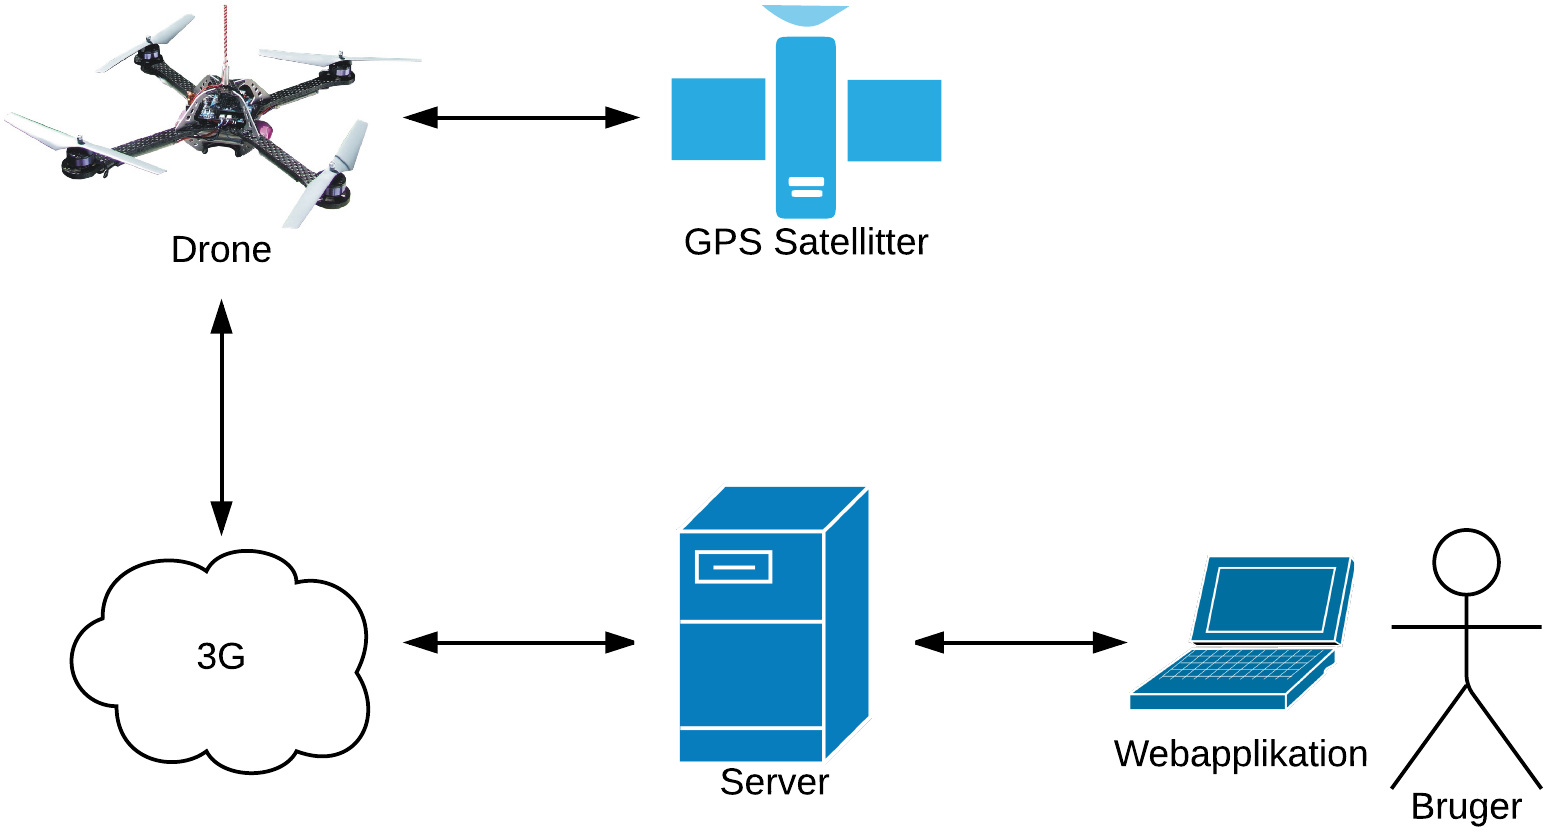
\includegraphics[width=1\textwidth]{Billeder/Projektbeskrivelse.png}
\vspace{-.5cm}
\caption{Systemskitse}
\label{fig:Systemskitse}
\end{figure}